\documentclass[12pt]{article}

\PassOptionsToPackage{backend=biber, style=numeric, sorting=none}{biblatex}

\usepackage{paper,math}

\usepackage[T2A]{fontenc}
\usepackage[utf8]{inputenc}
\usepackage[russian,english]{babel}
\usepackage{csquotes}

% For algorithm representation
\usepackage{algorithm}
\usepackage{algpseudocode} % or \usepackage{algorithmic}

% For pretty tables
\usepackage{booktabs}
\usepackage{caption}


\addbibresource{references.bib}

\hfuzz=30pt % Suppresses warnings for lines up to 20pt too wide
\sloppy

\title{Title}
\author{
  Мельничук Михаил\\ {\itshape\large Университет ИТМО}
}
\date{\today}

\booltrue{INCLUDECOMMENTS}
\newcommand{\kyle}[1]{\coauthorComment[Kyle]{#1}}

\graphicspath{{Melnichuk_Figs/}}
\captionsetup[figure]{name=Fig.}

\begin{document}

% ##################################################################################################
% Title Page
\maketitle
\begin{abstract}
  Abstract text

  \par\vspace{-2.5mm}
\end{abstract}

\newpage

% ##################################################################################################
\section{Introduction}

To be written later.

% ##################################################################################################
\section{Model}

The paper \cite{Melnichuk2026Analysis} provided an experimental testbed designed to emulate a queuing system within the currently used containerized orchestration framework of Kubernetes. The system architecture, as shown in Figure \ref{fig:Experimental_Setup}, consists of a dedicated Proxmox hypervisor server (with its own hardware) hosting a Kubernetes cluster with two nodes (one primary and one secondary node). The above setup ensures resource isolation and repeatability. A continuous stream of incoming requests, assumed to follow a Poisson process with intensity $\lambda$, is directed to the cluster. The Load Balancer is then responsible for distributing the request stream in a Round Robin manner.

The core microservice was implemented as a single, stateless Docker container image capable of processing both request types: CPU bound and I/O bound inquiries all with service time. The system is scaled horizontally by instantiating n identical replicas (pods/microservices) of this container, which function as $n$ homogeneous servers in the model. The Kubernetes scheduler was responsible for distributing these pods across the available cluster nodes.

\begin{figure}[!htbp]
  \centering
  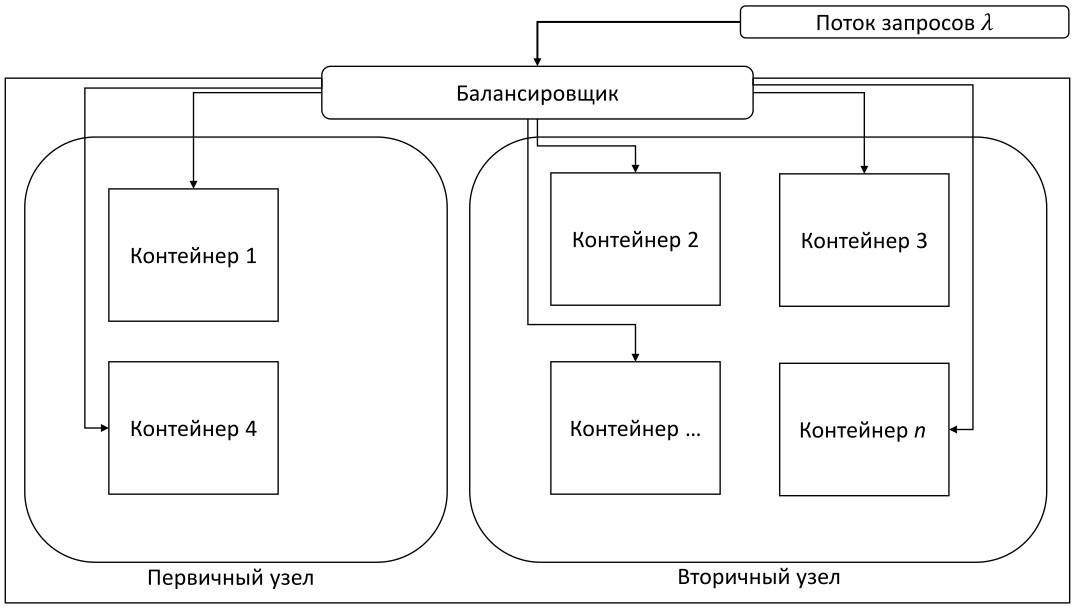
\includegraphics[height=5cm]{Experimental_Setup.jpeg}
  \caption{Experimental setup with a two-node Kubernetes cluster hosted on a dedicated Proxmox server. The cluster includes a Load Balancer for request distribution and stateless microservice containers that process incoming requests.}
  \label{fig:Experimental_Setup}
\end{figure}

The system was modeled as a queue with a state transition diagram illustrated in Figure \ref{fig:State_Transition_Graph}. Each state $S_i$ denotes the presence of $i$ requests in the system. The queue is unlimited, which means that the number of requests in the system can be less or more than the number of containers.

\begin{figure}[!htbp]
  \centering
  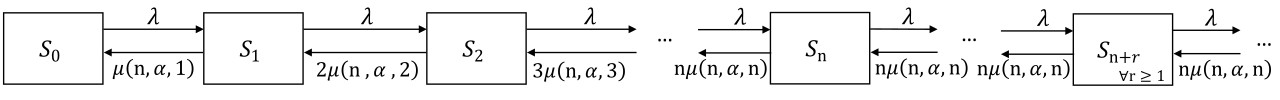
\includegraphics[height=1.3cm]{State_Transition_Graph.jpeg}
  \caption{State transition diagram of the system investigated.}
  \label{fig:State_Transition_Graph}
\end{figure}

The workload was characterized by a mixed distribution of requests. The key independent variable in this study was alpha ($\alpha$), defined as the proportion of requests that are CPU bound. Consequently, the proportion of I/O bound requests was ($1-\alpha$).

The arrival process followed a Poisson distribution with intensity $\lambda$ and the service rate $\mu(n,\alpha, i)$ was a function of $n$ (number of containers), $\alpha$ (proportion of CPU bound requests), and $i$ (number of requests present in system).

The stationary state is guaranteed when $\lambda < n\mu(n, \alpha)$, otherwise the queue size will infinitely grow.

The probability of finding the system empty (with zero requests) $p_0$:
\begin{equation}
  p_0=\left(
  1
  + \sum_{w=1}^{n}\left(\frac{\lambda^w}{w! \prod_{i=1}^{w}\mu\left(n,\alpha,i\right)}\right)
  +\frac{\lambda^{n+1}}{n! \prod_{i=1}^{n}\mu\left(n,\alpha,i\right) \left(n\mu\left(n,\alpha,n\right)-\lambda\right)}
  \right)^{-1};
  \label{eq:p0}
\end{equation}

Вероятность присутствия $i$ запросов в системе $p_k$:
\begin{equation}
  p_i = \left\{ \begin{array}{ll}
    \frac{\lambda^{i}}{i! \prod_{i=1}^{i}\mu\left(n,\alpha,i\right)} \, p_0                                                & \text{for } i \leq n, \\[11pt]
    \frac{\lambda^{i}}{n! \prod_{i=1}^{n}\mu\left(n,\alpha,i\right) \left(n\mu\left(n,\alpha,n\right)\right)^{i-n}} \, p_0 & \text{for } i > n.
  \end{array} \right.
  \label{eq:p_k}
\end{equation}

Вероятность того, что хотя бы один запрос находится в очереди $p_Q$
\begin{equation}
  p_Q=\frac{\lambda^{n+1}} {n! \prod_{i=1}^{n}\mu\left(n,\alpha,i\right) \left(n\mu(n,\alpha,n)-\lambda\right)} p_0.
  \label{eq:p_Q}
\end{equation}


Среднее число запросов, находящихся на обслуживание $L_N$ и в очереди $L_Q$, найдем в виде:
\begin{equation}
  L_N = \sum_{w=1}^{n} \frac{w\lambda^w}{w!\prod_{i=1}^{w}\mu\left(n,\alpha,i\right)} p_0
  +\frac{\lambda^{n+1}}{\left(n-1\right)! \prod_{i=1}^{n}\mu\left(n,\alpha,i\right) \left(n\mu\left(n,\alpha,n\right)-\lambda\right)} p_0
\end{equation}

\begin{equation}
  L_Q=\frac{\lambda^{n+1}} {\left(n-1\right)! \prod_{i=1}^{n-1}\mu\left(n,\alpha,i\right)\left(n\mu\left(n,\alpha,n\right)-\lambda\right)^2} p_0
\end{equation}

Среднее общее время нахождения в системе $T$ составляет:
\begin{align}
  T & = \frac{L_N + L_Q}{\lambda}= \sum_{w=1}^{n} \frac{w\lambda^{w-1}}{w!\prod_{i=1}^{w}\mu\left(n,\alpha,i\right)} p_0 + \nonumber                                                                                                          \\
    & + \frac{\lambda^n}{\left(n-1\right)! \prod_{i=1}^{n}{\mu\left(n,\alpha,i\right) \left(n\mu\left(n,\alpha,n\right)-\lambda\right)}}\left(1+\frac{\mu\left(n,\alpha,n\right)}{\left(n\mu\left(n,\alpha,n\right)-\lambda\right)}\right)p_0
  \label{eq:T}
\end{align}


%##################################################################################################
\section{Results}


\subsection{Recurrence without Factorials}
To make numerical stability possible, we define:
\[
  A_w = \frac{\lambda^w}{w! \prod_{i=1}^{w}\mu(n,\alpha,i)}, \quad k = 0, 1, 2, \dots
\]
This makes possible computing \(A_k\) iteratively:
\[
  A_0 = 1, \qquad A_{k+1} = A_k \cdot \frac{\lambda}{(w+1)\mu(n,\alpha,w+1)}.
\]

The method makes values of \(A_w\) stay within a reasonable range because (1) eliminates recalculation of (i) factorial, (ii) $\lambda^w$ and (iii) $\prod_{i=1}^{w}\mu(n,\alpha,i)$ for each step (2) each step is a simple multiplication and division. This way $A_k$ monotonically decays/grows without overflowing.

Using this optimization on modern computers allowed simulation and processing of up to $n \le 1000$ was still within `float` range, where without it no more than 250 containers.


\section{The problem of extracting Effective Service Rate from the container}

This is the place to explain why the estimation of method 1 is inconsistent with the total round time.

\begin{figure}[!htbp]
  \centering
  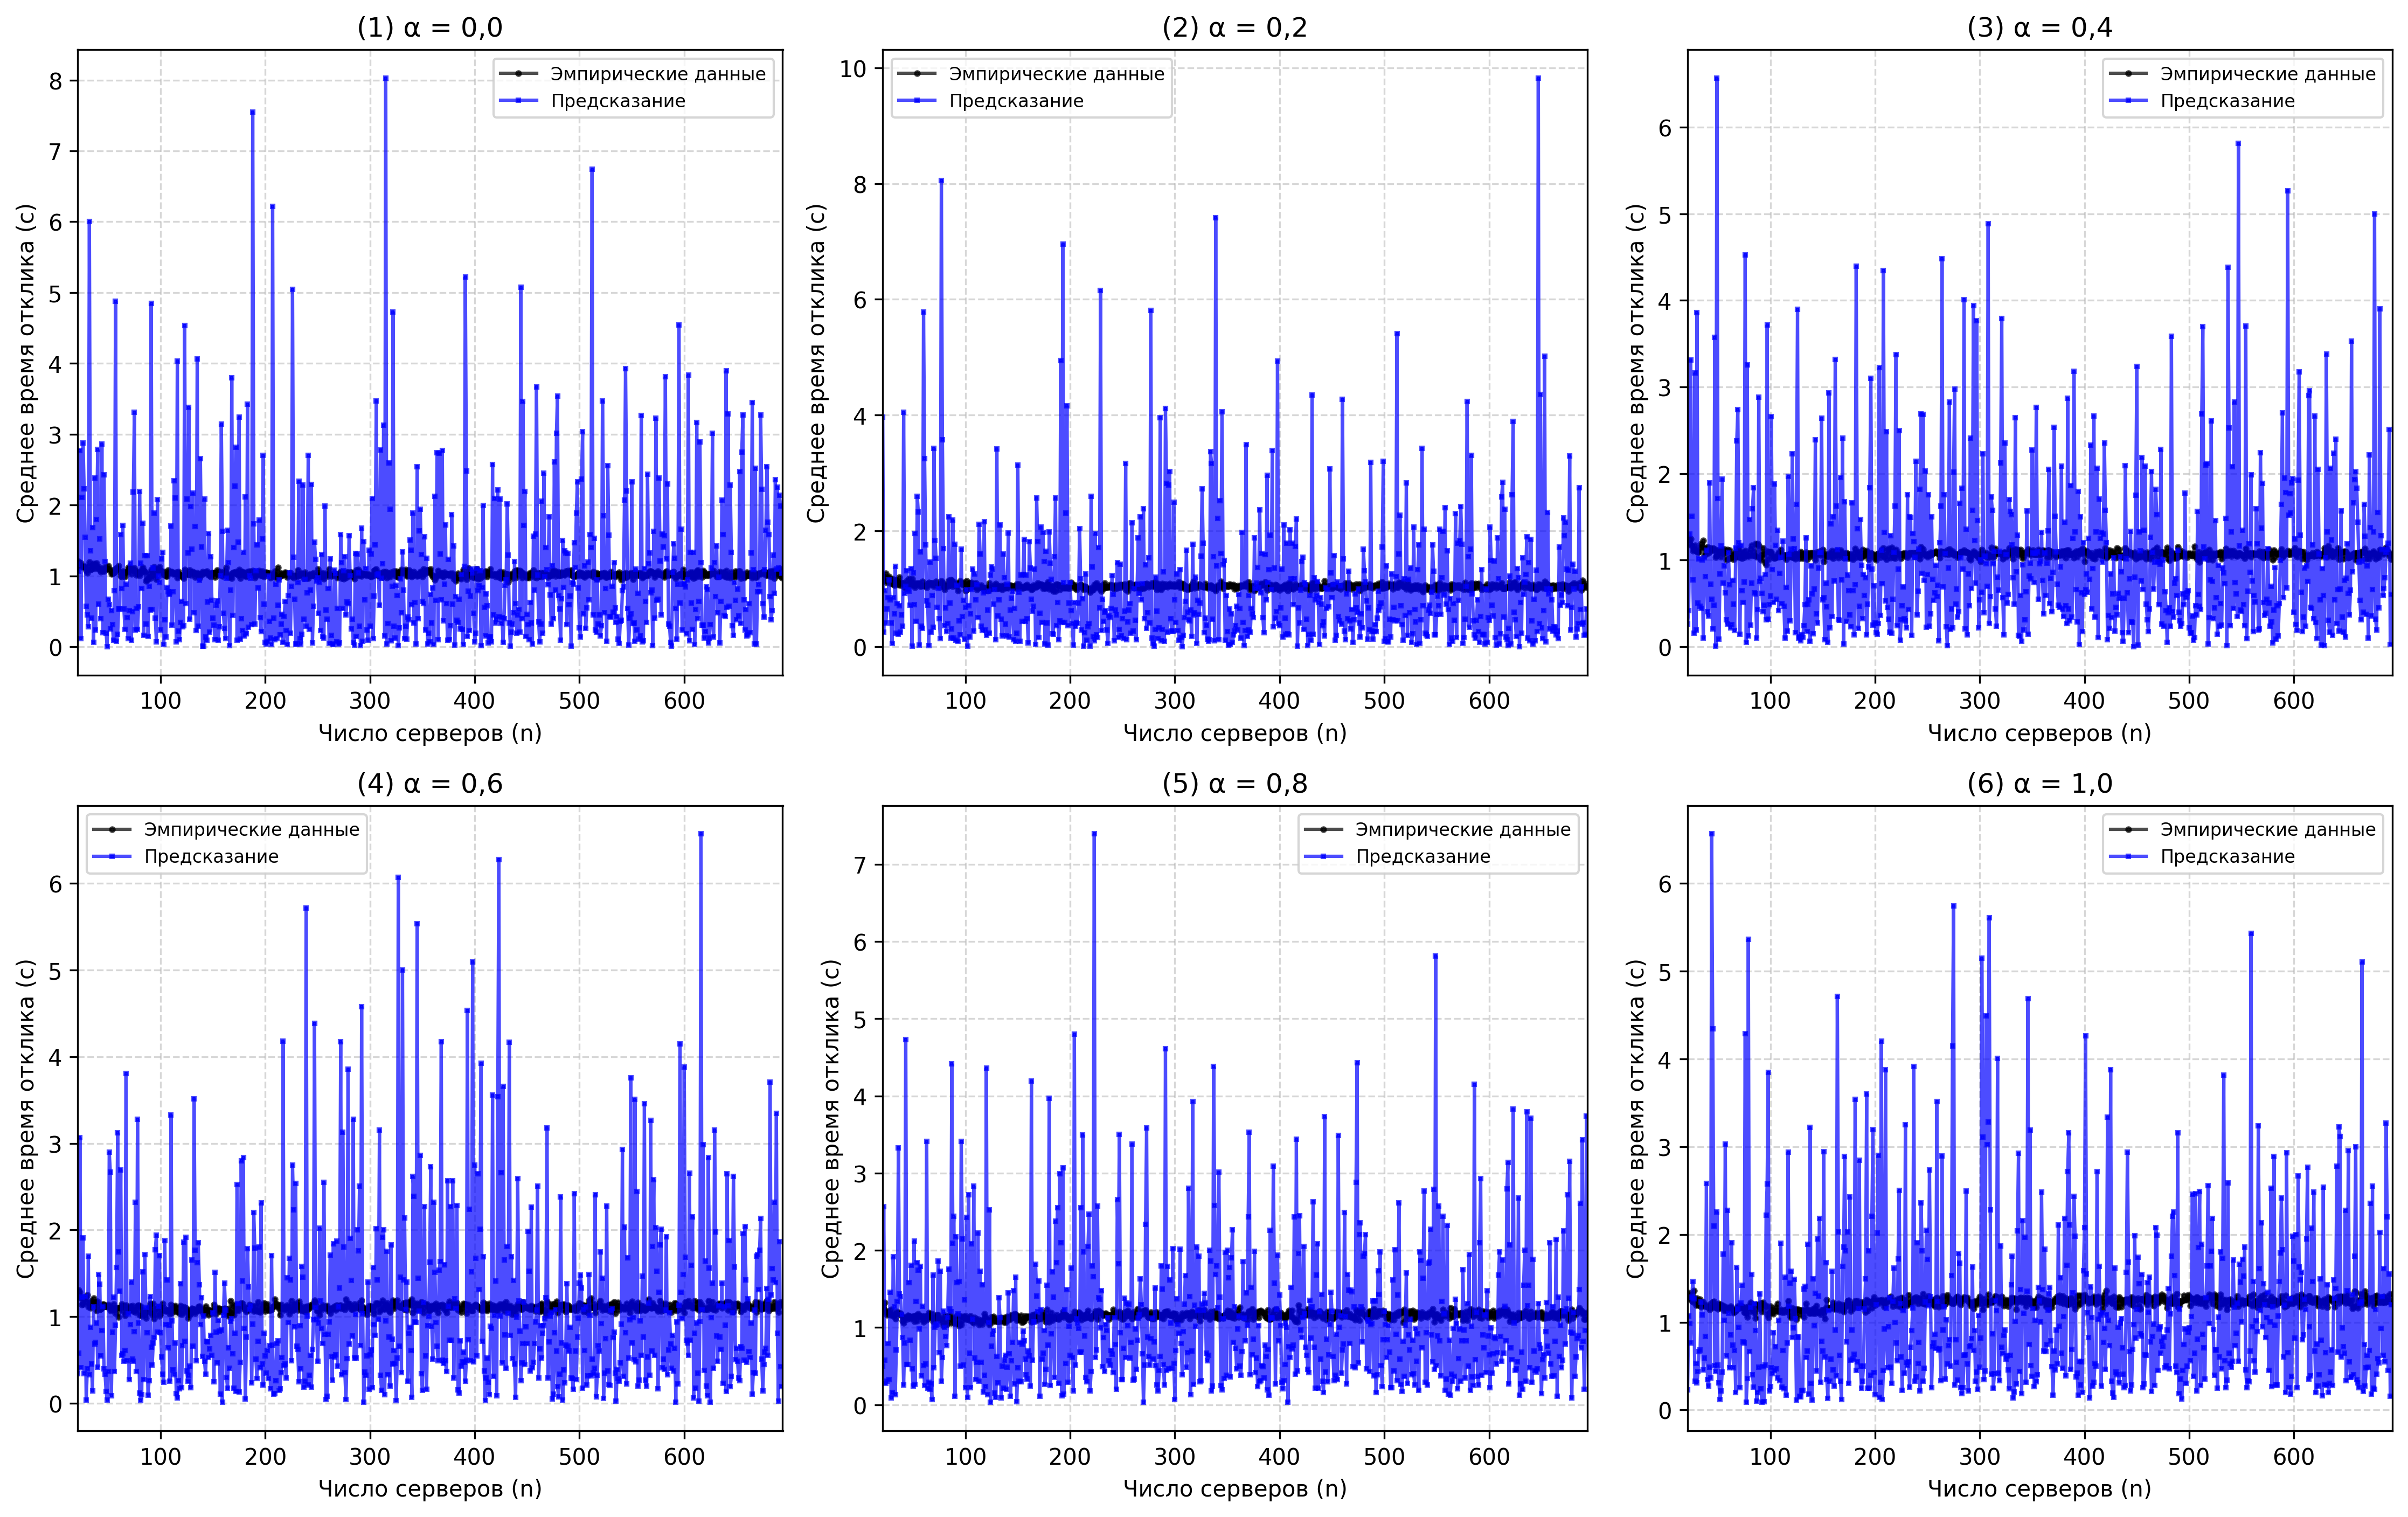
\includegraphics[height=10cm]{naive_mu_prediction.png} \\
  \caption{Аналитическое моделирование системы на основе среднего времени обслуживания измеренного в контейнерах}
  \label{fig:naive_mu_prediction}
\end{figure}

The problem is that on the container level one does not feel the overheads associated with waiting in the queue and load balancing.

\begin{table}[htbp]
  \centering
  \caption{Model Performance Metrics per $\alpha$}
  \label{tab:model_metrics}

  % Adds a little vertical breathing room between rows
  \renewcommand{\arraystretch}{1.2}

  \begin{tabular}{c r r r}
    \toprule
    $\alpha$         & \multicolumn{1}{c}{RMSE} & \multicolumn{1}{c}{MAE} & \multicolumn{1}{c}{MAPE (\%)} \\
    \midrule
    0.0              & 1.0909                   & 0.7821                  & 75.8992                       \\
    0.2              & 1.1204                   & 0.7725                  & 73.8104                       \\
    0.4              & 0.9573                   & 0.7093                  & 65.9469                       \\
    0.6              & 1.0069                   & 0.7382                  & 66.5865                       \\
    0.8              & 0.9388                   & 0.7013                  & 60.7633                       \\
    1.0              & 1.0028                   & 0.7644                  & 62.5456                       \\
    \midrule
    % Bold the average row to make it stand out
    \textbf{Average} & \textbf{1.0195}          & \textbf{0.7446}         & \textbf{67.5920}              \\
    \bottomrule
  \end{tabular}

  \vspace{0.5em}

  % Footer summary text
  \noindent\footnotesize Average RMSE: 1.0195 \quad | \quad Average MAE: 0.7446 \quad | \quad Average MAPE: 67.5920\%
\end{table}

\subsection{Practical Estimation of Effective Service Rate}

% To analytically validate the proposed queuing model,  the service rate $\mu(n, \alpha, i)$ is estimated for each $(n, \alpha, i)$ by the algorithm \ref{alg:mu_eff_pseudo}, where $T_{\text{emp}}^{n, \alpha}(i)$ is the measured mean service time when the system had exactly $i$ requests in the system based on the empirical data gathered from the experimental testbed. The continuous service rate function derived from this approach is then explicitly utilized as the intensity (rate parameter) of the Poisson process governing the service times. Because this updated service rate is derived from end to end empirical measurements, this approach implicitly accounts for all unpredictable overheads like Kubernetes scheduling jitter, load-balancer forwarding delays, network latency, OS interference, and variable processing speeds, and the specific performance impact of the workload mix $\alpha$.

Для того чтобы аналитически проверить предложенную модель СМО $\mu(n, \alpha, i)$ для каждого состояния нужно выявить $(n, \alpha, i)$. где $T_{\text{emp}}^{n, \alpha}(i)$ — это измеренное мэн сервис тайм, когда система имела ровно $i$ реквестов, на базе эмпирикал дат, гезеренных с экспериментального тестбеда. Континуальная функция сервис рейта, деривированная из этого аппроча, затем эксплицитно утилизится как интенсивность (рейт параметр) Пуассоновского процесса, управляющего сервис таймами. Потому что этот апдейтед сервис рейт деривирован из энд-ту-энд эмпирикал мэжурментов, данный аппроч имплицитно акаунтит все непредсказуемые оверхеды, такие как скедулинг джиттер Kubernetes, дилейс форвардинга лоад-балансера, сетевая латентность, интерферен от ОС, и вариативные процессинг спидс, а также специфическое перфоманс влияние ворклоад микса $\alpha$.

Идея предложенной кусочно заданной формулы приближения времени обслуживания \ref{eq:mu_eff} заключается в том, чтобы включить в себя все непредсказуемые задержки, такие как сетевая нагрузка, обработка прокси и задержки планирования Kubernetes в одну единственную, калиброванную скорость обслуживания $\mu(n, \alpha, i)$ при $i$ запросов в системе, $n$ контейнеров и параметра $\alpha$.

Когда $i \le n$, количество запросов $i$ меньше или равно числу серверов $n$. В этом сценарии очередь не формируется, и запрос идет напрямую к свободному серверу. Поэтому, эффективный $\mu$ это просто инверсия от среднего эмпирического времени обслуживания $T_{\mathrm{emp}}^{n, \alpha}(i)$.

При $i > n$ все сервера заняты и формируется очередь. В данном случае $T_{\mathrm{emp}}^{n, \alpha}(i)$ теперь включает в себя не только чистое время обработки запроса, но и ожидание в очереди и других задержек сети, балансировщика и Kubernetes.  Опираясь на свойство отсутсвия памяти Пуассоновского процесса, мы знаем, что для $i$ запросов, которые обрабатываются параллельно на $n$ серверах, математически выражается как $i / (n \cdot T_{\mathrm{emp}}^{n, \alpha}(i))$.

\begin{equation}
  \mu_{\mathrm{eff}}(n, \alpha, i) =
  \left\{
  \begin{array}{ll}
    \dfrac{1}{T_{\mathrm{emp}}^{n, \alpha}(i)},         & \text{if } i \le n, \\[12pt]
    \dfrac{i}{n \cdot T_{\mathrm{emp}}^{n, \alpha}(i)}, & \text{if } i > n.
  \end{array}
  \right.
  \label{eq:mu_eff}
\end{equation}

% \begin{algorithm}
%   \caption{Estimation of Effective Service Rate $\mu_{\text{eff}}(n, \alpha, i)$}
%   \label{alg:mu_eff_pseudo}
%   \begin{algorithmic}[1]
%     \Require Number of servers $n$, state $i$, empirical time array $T_{\text{emp}}^{n, \alpha}$ measured for a given $(n, \alpha)$
%     \Ensure Effective service rate $\mu_{\text{eff}}$
%     \If{$i \le n$} \Comment{No queue}
%     \State $\mu_{\text{eff}} \gets \frac{1}{T_{\text{emp}}^{n, \alpha}(i)}$
%     \Else \Comment{All servers busy}
%     \State $\mu_{\text{eff}} \gets \frac{i}{n \cdot T_{\text{emp}}^{n, \alpha}(i)}$
%     \EndIf
%     \State \Return $\mu_{\text{eff}}$
%   \end{algorithmic}
% \end{algorithm}
% do not specify the degree of the polynomial or how you prevent overfitting (e.g., cross validation, regularization)

\begin{table}[htbp]
  \centering
  \caption{Model Performance Metrics per $\alpha$}
  \label{tab:model_metrics}

  % Adds a little vertical breathing room between rows
  \renewcommand{\arraystretch}{1.2}

  \begin{tabular}{c r r r}
    \toprule
    $\alpha$         & \multicolumn{1}{c}{RMSE} & \multicolumn{1}{c}{MAE} & \multicolumn{1}{c}{MAPE (\%)} \\
    \midrule
    0.6              & 0.0690                   & 0.0547                  & 4.9324                        \\
    0.0              & 0.0669                   & 0.0522                  & 5.0549                        \\
    0.2              & 0.0766                   & 0.0600                  & 5.7290                        \\
    1.0              & 0.0790                   & 0.0598                  & 4.8543                        \\
    0.8              & 0.0702                   & 0.0567                  & 4.9037                        \\
    0.4              & 0.0669                   & 0.0514                  & 4.7523                        \\
    \midrule
    % Bold the average row to make it stand out
    \textbf{Average} & \textbf{0.0714}          & \textbf{0.0558}         & \textbf{5.0378}               \\
    \bottomrule
  \end{tabular}

  \vspace{0.5em}

  % Footer summary text
  \noindent\footnotesize Average RMSE: 0.0714 \quad | \quad Average MAE: 0.0558 \quad | \quad Average MAPE: 5.0378\%
\end{table}

\subsection{Simulation Modeling of the queuing system}
In addition to the analytical method, simulation modeling was conducted to validate the results using SimPy library in python.

% the simulation uses the fitted exponential service times, the actual measured service time distribution, or a state dependent service time model

% You must specify the number of replications per configuration, the simulation warm up period, and the confidence intervals for your metrics. Without this, the "validation" is not statistically rigorous.


A full factorial experimental design was employed with parameters that were chosen to ensure that the system transitioned from under provisioned to over provisioned for sufficiently long observation window:
- Arrival rate $\lambda = 1$.
- Exponential service times ????.
- Number of containers $n \in [1, 300]$.
- Workload mix alpha $\alpha \in {0, 0.2, 0.4, 0.6, 0.8, 1}$.
- Independent and identically distributed service times across servers.


\begin{figure}[!htbp]
  \centering
  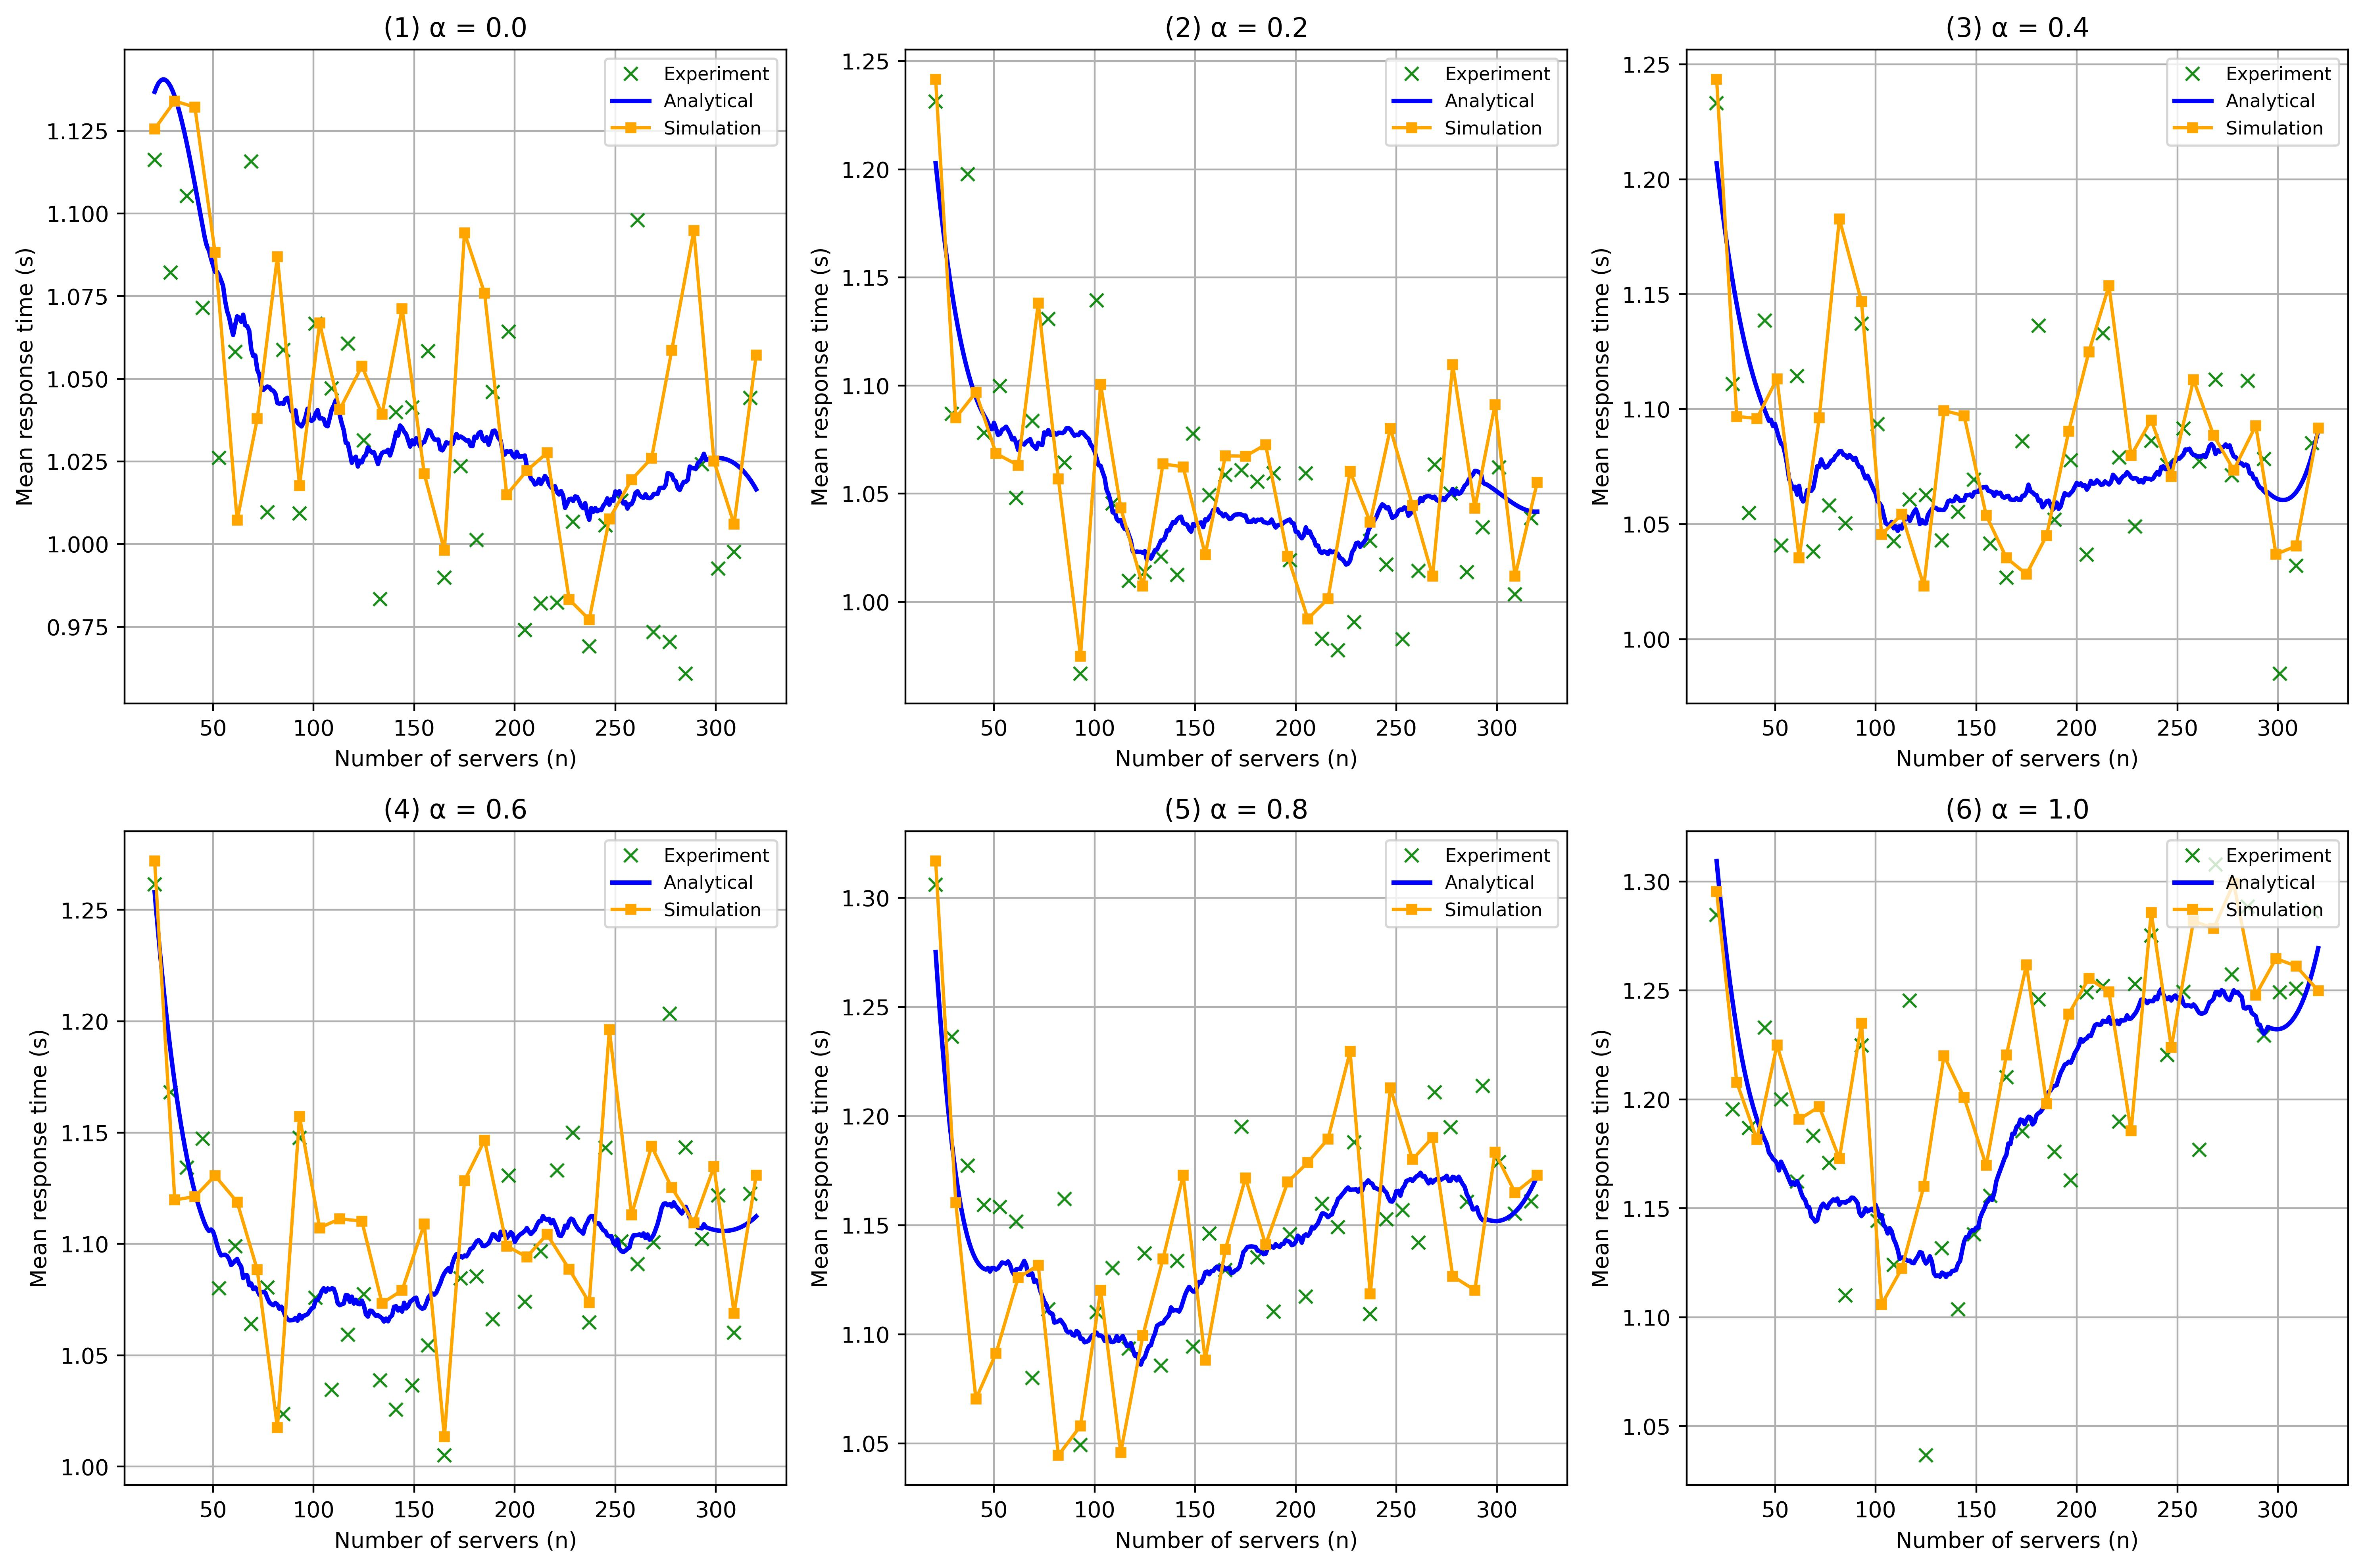
\includegraphics[height=10cm]{Experimental_Analytical_Simulation.jpeg} \\
  \caption{Симуляционное моделирование (оранжевая линия с точками), аналитическое вычисление (синяя сплошная линия) и экспериментально полученные данные на сервере Kubernetes (зелёные х). В связи в тяжестью вычисления $k!$ количество контейнеров уменьшено до 300.}
  \label{fig:Mel_fig_System_States}
\end{figure}

% ##################################################################################################
\section{Discussion}
To be written later.

% ##################################################################################################
\section{Conclusion}

To be written later.

% ##################################################################################################
\printbibliography[title={References}]

\end{document}